%%%%%%%%%%%%%%%%%%%%%%%%%%%%%%%%%%%%%%%%%
% Stylish Article
% LaTeX Template
% Version 2.1 (1/10/15)
%
% This template has been downloaded from:
% http://www.LaTeXTemplates.com
%
% Original author:
% Mathias Legrand (legrand.mathias@gmail.com) 
% With extensive modifications by:
% Vel (vel@latextemplates.com)
%
% License:
% CC BY-NC-SA 3.0 (http://creativecommons.org/licenses/by-nc-sa/3.0/)
%
%%%%%%%%%%%%%%%%%%%%%%%%%%%%%%%%%%%%%%%%%

%----------------------------------------------------------------------------------------
%	PACKAGES AND OTHER DOCUMENT CONFIGURATIONS
%----------------------------------------------------------------------------------------
\documentclass[10pt]{SelfArx} % Document font size and equations flushed left

%fleqn,
\usepackage[T1]{fontenc}
\usepackage{newtxmath,newtxtext}

\usepackage{textcomp}
\usepackage{gensymb}

\usepackage{amsmath, amsfonts}

\usepackage{titlesec}
\usepackage{subfigure}
%\titlespacing*{\section}{-0.5pt}{0.5\baselineskip}{\baselineskip}
%\usepackage[english]{babel} % Specify a different language here - english by default

%----------------------------------------------------------------------------------------
%	COLUMNS
%----------------------------------------------------------------------------------------

\setlength{\columnsep}{0.55cm} % Distance between the two columns of text
\setlength{\fboxrule}{0.75pt} % Width of the border around the abstract

%----------------------------------------------------------------------------------------
%	COLORS
%----------------------------------------------------------------------------------------

\definecolor{color1}{RGB}{0,0,90} % Color of the article title and sections
\definecolor{color2}{RGB}{0,20,20} % Color of the boxes behind the abstract and headings

%	HYPERLINKS
%----------------------------------------------------------------------------------------

\usepackage{hyperref} % Required for hyperlinks
\hypersetup{hidelinks,colorlinks,breaklinks=true,urlcolor=color2,citecolor=color1,linkcolor=color1,bookmarksopen=false,pdftitle={Title},pdfauthor={Author}}

%----------------------------------------------------------------------------------------
%	ARTICLE INFORMATION
%----------------------------------------------------------------------------------------

\JournalInfo{Tanzanian Ministry of Water} % Journal information
\Archive{December 5, 2016} % Additional notes (e.g. copyright, DOI, review/research article)

\PaperTitle{Predicting Water Well Functionality} % Article title


\Authors{Alexis Rouge Carrassat (amr439), Anthony Niznik (an533),  Fan Liu (fl379)} % Authors

\Keywords{} % Keywords - if you don't want any simply remove all the text between the curly brackets
\newcommand{\keywordname}{Keywords} % Defines the keywords heading name

%----------------------------------------------------------------------------------------
%	ABSTRACT
%----------------------------------------------------------------------------------------

\Abstract{The country of Tanzania is currently facing a water supply challenge. Water wells are not fixed quickly, leading to thousands of people not having access to a clean water supply. The Tanzanian Ministry of Water is trying to determine whether water wells are functional, functional - in need of repair, or non-functional without having someone go to the well physically to check. The Ministry has requested the creation of a model that is able to determine which water wells are functional and which ones are in need of repair.}

%----------------------------------------------------------------------------------------

\newlength\tindent
\setlength{\tindent}{\parindent}
\setlength{\parindent}{0pt}
\renewcommand{\indent}{\hspace*{\tindent}}

\begin{document}



\flushbottom % Makes all text pages the same height

\noindent \maketitle % Print the title and abstract box  


\tableofcontents % Print the contents section

\thispagestyle{empty} % Removes page numbering from the first page

%----------------------------------------------------------------------------------------
%	ARTICLE CONTENTS
%----------------------------------------------------------------------------------------

\section{Exploratory Data Analysis} % The \section*{} command stops section numbering
\subsection{Data Characteristics}

The data set comprises of a variable matrix with 39 features and 59,400 rows of water wells. The output we wish to predict is whether a water well is functional, non-functional, or functional-needs repair. The following are the number of columns (features) by type: 7 continuous, 27 categorical, 2 binary, 2  with all of the same value, and 1 date. Some continuous variables include \textit{longitude}, \textit{latitude}, \textit{GPS height} (altitude of well), and \textit{date\_recorded} of the well. Please see Tables 1 and 2 to get a feel for the structure of the data set.
\break

\begin{table*}[t]
  \centering
\caption{Data set example}
\begin{tabular}{ |c|c|c|c|c|c|c|c|c|c| }
      \hline
      amount\_tsh & date\_recorded & gps\_height & installer & \ldots & longitude & latitude & status\_group\\
      \hline
      \hline
      6000.0 & 3/14/11 & 1390 & Roman & \ldots & 34.938093 & -9.856322 & functional\\
      0.0 & 3/16/13 & 1399 & GRUMETI & \ldots & 34.698766 & -9.856322 & functional\\
      25.0 & 2/23/13 & 576 & Roman & \ldots & 37.460664 & -9.856322 & functional\\
      0.0 & 1/28/13 & 263 & UNICEF & \ldots & 38.486161 & -11.155298 & non-functional\\
      \hline
    \end{tabular}
  \label{tab:1}
\end{table*}

There were plenty of missing values and questionable zero values in columns. We had 3,056 missing values in the \textit{permit} column and 3,622 missing in the \textit{funder} column. Incorrect zero values occurred in the \textit{longitude} column 1,812 times (Longitude Range: 29$^\circ$ E to 41$^\circ$ E) and 18,897 times in the \textit{construction year} column (all other years >1959). To get a sense of where all the water wells are located, we plotted the water wells on a geographical map with blue indicating the well is functional, and red indicating non-functional (see Figure 1). We see that wells form geographic clusters, especially around the coast and borders of Tanzania. In the next section, we discuss the insights obtained from visualizing the data.


\begin{figure}[ht]\centering
\captionsetup{skip=0.5cm}
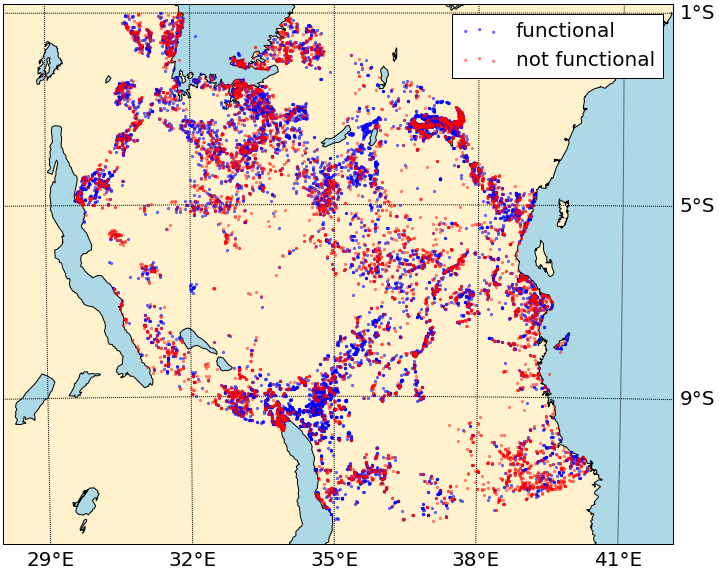
\includegraphics[width=\linewidth]{location.png}
\caption{Locations of wells in Tanzania}
\label{fig:map}
\end{figure}


\subsection{Data Visualization}

We first used histograms to visualize which variables could separate well functionality most distinctly. We found that whether a water well had a permit (legally authorized to exist) or not greatly affected the classification of the well. If a water well has a permit, it is much more likely to be functional than if it does not have a permit (see Figure 2 where a random sample of the data is plotted). This makes permit an important feature to include in our model.
\break

\begin{table*}[t]
  \centering
\caption{Summary statistics}
\begin{tabular}{ |c|c|c|c|c|c| }
      \hline
      Column Name & Mean & Standard Deviation & Minimum & Median & Maximum\\
      \hline
      \hline
      longitude & 35.98 & 2.56 & 29.61 & 36.65 & 40.3\\
      latitude & -6.24 & 2.76 & -11.65 & -6.06 & -1.04\\
      gps\_height & 1002.37 & 618.08 & -63.00 & 1154.00 & 2770.00\\
      \hline
  \end{tabular}
  \label{tab:2}
\end{table*}

\begin{figure}[ht]\centering
\captionsetup{skip=0.5cm}
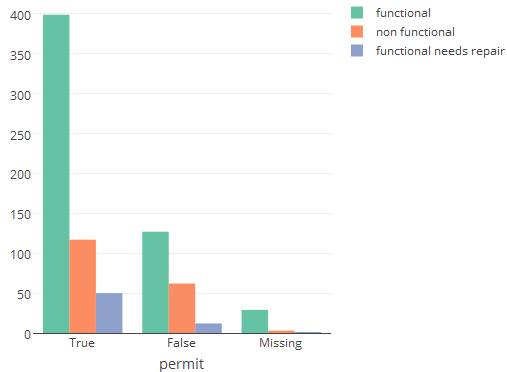
\includegraphics[width=\linewidth]{permit.png}
\caption{Number of wells based on permit}
\label{fig:permit}
\end{figure}

Another question to address includes the following: how does the variability in continuous variables depend on the functionality of the well? We considered the variable \textit{GPS Height}, which gives the height of the water well relative to sea level in meters (see Figure 3). We created a boxplot that displays the spread of the GPS Height for functional, non-functional, and functional-needs repair wells (see Figure 5). We see that the median GPS height of non-functional wells is slightly lower than the median of both functional and functional-needs repair wells. This implies that non-functional wells tend to have a lower GPS height than the other wells. Please note that the boxplot contains all values except for water wells at zero altitude because of our suspicion of corrupt entries (see Figure 4 and Section 1.4 for more details).
\break

\begin{figure}[ht]\centering
\captionsetup{skip=0.5cm}
\includegraphics[width=\linewidth]{histo1.png}
\caption{GPS height distribution (includes corrupt data)}
\label{fig:hitso1}
\end{figure}

\begin{figure}[ht]\centering
\captionsetup{skip=0.5cm}
\includegraphics[width=\linewidth]{histo2.png}
\caption{GPS height distribution (elevations corrected)}
\label{fig:hitso2}
\end{figure}

\begin{figure}[ht]\centering
\captionsetup{skip=0.5cm}
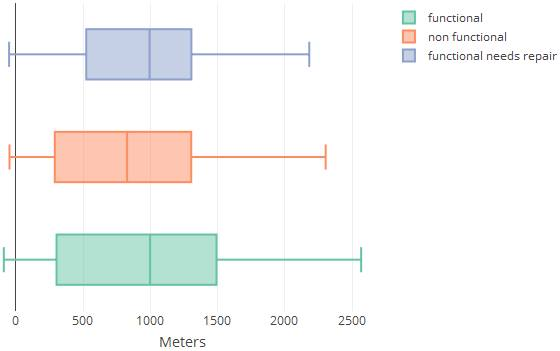
\includegraphics[width=\linewidth]{boxplot2.png}
\caption{Well classification based on GPS height}
\label{fig:GPS}
\end{figure}

While plotting different features, we quickly realized that longitude and latitude were both important features for classification. Though we plotted the water wells onto the map of Tanzania, we wanted to get a better idea of where most of the functional wells may be located. We created a plot of longitude vs latitude this time to see if we can get a better sense of where the functional wells were located. We pinpointed a rectangular area  in the center of Tanzania (shaded in blue) where over 70\% of wells are functional (see Figure 6 where a random sample of the data is plotted). This result proved consistent when plotting with different samples of the data.
\break

\begin{figure}[ht]\centering
\captionsetup{skip=0.5cm}
\includegraphics[width=\linewidth, height = 5.5cm]{map_color3.png}
\caption{Longitude vs latitude of wells; functional wells (blue), non-functional wells (red)}
\label{fig:map2}
\end{figure}

After this discovery, we considered the 21 regions in Tanzania and the percent of non-functional water wells in each region. When we created a bar plot that ordered the regions from lowest longitude (West) to highest longitude (East), left to right on the histogram, we found that the regions in the center of Tanzania (Iringa and Arusha) had the lowest percentages of non-functional wells (see Figure 7). This indicates that water wells in the center of Tanzania have a higher probability of being functional than wells farther west or east.

\begin{figure}[ht]\centering
\captionsetup{skip=0.5cm}
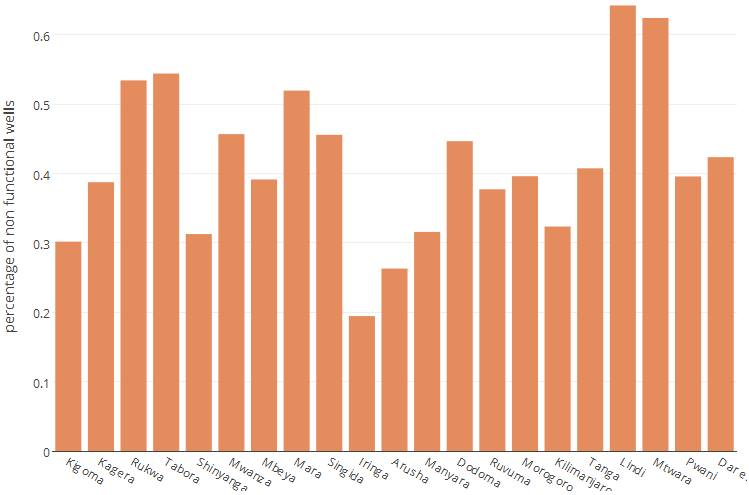
\includegraphics[width=\linewidth]{barplot2.png}
\caption{Barplot of percent of non-functional wells based on regions that are ordered by longitude (left to right)}
\label{fig:barplot}
\end{figure}

\begin{figure*}
\centering
\begin{minipage}[b]{.4\textwidth}
\captionsetup{skip=0.5cm}
\includegraphics[width=\linewidth, height = 5.8cm]{topo.png}
\caption{Elevation map of Tanzania (in meters)$^{[1]}$}\label{label-a}
\end{minipage}\qquad \qquad \qquad
\begin{minipage}[b]{.4\textwidth}
\captionsetup{skip=0.5cm}
\includegraphics[width=\linewidth]{gpsheight.png}
\caption{Geography of GPS height of well}\label{label-b}
\end{minipage}
\end{figure*}

\subsection{Cleaning the Data}

\subsubsection{Dates}

We immediately left out of our model any columns that had the same value for more than 95\% of their row values (2 features fit this description, \textit{recorded by} and \textit{number private}). Then, we changed the column that had calendar date of water well status check (day, month, year) to just the number of days from the current date to the earliest date of water well status check. So, if the earliest date any well was checked is 10/14/2002, then a well checked on 12/03/2013 would have 4,069 as its value. We also created two new binary columns, one column to indicate whether the water well was checked in the dry season and one column to indicate whether the water well was checked in the wet season. The dry season include the months from June to October and the wet season includes months from November until May.
\break

\subsubsection{Many Unique Values}

We also transformed the \textit{installer} column (which company installed the well). Since there are 2,113 unique installer values and most rows belonged to the top two installers (See Table 3), we simply created three new binary variables (one for the installer with the most wells, one for the installer with the second most wells, all other installers placed in a \textit{other} column, and a column for missing values discussed in the next paragraph).
\break

\begin{table*}[t]
  \centering
\caption{Category Frequency}
\begin{tabular}{ |c|c|c|c|c| }
      \hline
      Column Name & \# Categories & Most Frequent & Frequency & \# Missing\\
      \hline
      \hline
      installer & 2113 & DWE & 16255 & 3636\\
      region & 21 & Iringa & 5294 & 0\\
      water\_quality & 8 & soft & 50818 & 0\\
      \hline
    \end{tabular}
  \label{tab:3}
\end{table*}

\subsubsection{One-Hot Encoding}

For the categorical variables, we used one-hot encoding to change a variable of one column and d distinct values to d binary variable columns. This increased the number of categorical columns of our model to 226 columns. If values were missing from a particular column, we created a new binary variable that takes one if a value is missing and zero otherwise. In this way, we could retain some information, even for missing values and not have to delete an entire row just for 1 missing value.  For logistic regression, we standardized continuous variables such as longitude and latitude of water well since regularized least squares is not scaling invariant. We standardized the data by subtracting the column mean of each column and then dividing by the standard deviation of each column for all continuous variables.

\subsection{Corrupt Data}

\subsubsection{GPS Height}

We noticed for the variable GPS height that the distribution of classification (functional, non-functional) is very different for the wells with zeros and the wells with a value not zero. We decided to plot the GPS height based on the longitude and latitude of each water well. We did this so that we could see where water wells are classified as having zero altitude to determine if they actually should be at zero altitude (see if they are corrupt). When we plotted the altitude of wells (see Figure 9), we found a big cluster of wells at zero altitude in the northwest part of Tanzania. When we compared this to the topography of Tanzania (see Figure 8), we found that the northwest region of Tanzania is about 1000 meters above sea level. This means that the water wells with GPS height of zero that are located in the northwestern part of Tanzania are incorrect and therefore corrupt. 
\break

\subsubsection{Correcting Elevations}
We verified using the Google Maps API that indeed most water wells that were assigned a GPS height of zero in the data set were at a higher elevation. To correct this corruption, we looked to substitute the incorrect zeros with the correct elevation using the Google Maps API. Since Google has a usage limit of 2,500 free requests per day$^{[2]}$ (and our data contains about 20,000 incorrect zeros), we decided to group the latitude and longitude into 1,600 squares. We did this by taking the range of latitude values that Tanzania spreads across and dividing that range by 40. We then did the same for longitude. With the 40 by 40 matrix, we were able to place 1,600 points on the area that encompasses Tanzania. With these points, we assigned each well to the point it should belong to by checking which point creates the minimum distance between the point and the well. With these assignments, we replaced the wrong elevation of wells with the new, approximate elevation assignment (See Figure 11 for more details).
\break


\subsubsection{Handling Zero Values in Population}

For population, we decided to add a binary variable column that indicates whether the population is zero or greater than zero since zero appears very often (33\% of the values are zero) and we do not have a means of verifying or substituting these values with more accurate ones. Additionally, the variance of population and GPS height are very high so we took the natural log of these variables to make sure that the values that are greater than zero but small will still have a significant impact on the model. This transformation is used for logistic regression and random forest which we will discuss in the next section.

\section{Model Selection}

\begin{figure*}
\centering
\begin{minipage}[b]{.4\textwidth}
\captionsetup{skip=0.5cm}
\includegraphics[width=\linewidth]{zeros.png}
\caption{Locations of wells with zero GPS height}\label{a}
\end{minipage}\qquad \qquad \qquad
\begin{minipage}[b]{.4\textwidth}
\captionsetup{skip=0.5cm}
\includegraphics[width=\linewidth, height = 5cm]{dots.png}
\caption{Points that assign new well elevations}\label{b}
\end{minipage}
\end{figure*}

\subsection{Logistic Regression}

For our initial model, we chose to use the logistic regression model (denoted by $h(x)$) because the water well problem is a classification problem. We first split the data into 70\% training set, 15\% validation set, and 15\% testing set. We did this by using the randomsplit function. Randomsplit first generates a list of random indices and then it matches those indices to the actual values of the original array. Then it assigns the appropriate percentages of this random, matched list to each set. We used the validation set to calculate the $\lambda$ that minimizes the percent of misclassifications. The objective function of logistic regression is defined as the following: 

\begin{equation}
 h(x) = log(1+e^{(-yw^Tx)}) + \lambda||w||_1
\end{equation}

Since we added many new variables with one-hot encoding, we chose $l_1$ for regularization because it encourages sparsity. Because logistic regression is a binary logistic model (1 if water well is a certain classification and 0 otherwise), we could not simply use one regression to perform the analysis. Instead, we created 3 different logistic regression models for each class i (one for each classification of functional, non-functional, and functional-needs repair). We then used that fact the logistic regression returns the probability that a water well is a certain classification to just simply take the maximum probability of the three models in order to classify the well (see Equation 2).

\begin{equation}
 y= \underset{i}{\mathrm{argmax}}\, h_i(x) 
\end{equation}

\subsection{Random Forest}

Another model we considered is random forest. The way random forest works is that it creates groups of decisions trees (x) where each tree is assigned a certain number of features at random (while using the whole training set). Each decision tree is split on each feature based on maximizing the amount of information we can gain from each split (create the greatest reduction in entropy). When it comes time to predict, a majority vote is taken from the decision trees to classify each water well (see Figure 12). So, if a water well is classified by 10 trees, and 7 trees classify the well as functional, 2 trees classify as non-functional, and 1 classifies the well as functional-needs repair, then the well will be classified as the majority vote which is functional. For more information about random forest, please refer to chapter 15 in the textbook,\textit{ The elements of statistical learning: Data mining, inference, and prediction.}$^{[3]}$
\break

\begin{figure}\centering
\captionsetup{skip=0.5cm}
\includegraphics[width=\linewidth]{rfreal.png}
\caption{Random forest example$^{[4]}$}
\label{fig:rf}
\end{figure}

For our random forest model, we used 100 trees in our forest. We allowed trees to grow to a maximum depth of 30 and allowed trees to randomly split n times (here n is equal to the square root of the number of features chosen to split on). Random forest is not prone to underfitting since decision trees tend to overfit due to the fact that they can keep splitting to get a training error near zero. Also, random forest is not prone to overfitting since our maximum depth is a form of regularization that prevents each single tree from overfitting. Majority vote also helps prevent overfitting because it prevents overfit trees from weighing heavily on the classification.

\section{Results}

To test the effectiveness of both models, we calculated accuracy as the percentage of correctly classified water wells in our test set by the models. We found that logistic regression was able to classify with an accuracy of about 73\%. On the other hand, random forest could classify with an astonishing 80\% accuracy. A reason that the accuracy of the test data is low for logistic regression may lie in the fact that the training error for logistic regression is also low (about 74\%) which implies that logistic regression has a relatively high bias.
\break

When we replaced the incorrect elevations of water wells with more accurate elevations, we found that our accuracy increased a whole percentage to 81\%! The significant impact of changing the incorrect zero values to a better approximation of elevation makes sense since the corrupted data affected over one third of the data set.

\section{Conclusion}

By using techniques we learned in class such as one-hot encoding, logistic regression, and regularization, we were able to classify the functionality of water wells in Tanzania fairly well with 73\% accuracy. Since logistic regression is a linear model, it is not able to capture the inherit phenomena in the data set especially for continuous variables (such as latitude and longitude) because one can not necessarily create a line to separate functional and non-functional wells based on location. With random forest, we were able to achieve an accuracy of 81\%. 
\break

We are fairly confident that our model will be able to generalize to new well data because random forest is very flexible and can adjust itself since it takes samples of the features to split upon. One thing to note is that we found longitude and latitude to be significant features in determining classification of water wells so if a new data set comes in without these features, our model may perform poorly. Also random forest is not as interpretable as logistic regression, so The Tanzanian Ministry of Water may prefer to use the logistic model since fewer variables can explain the classification of each water well. The Ministry will find our model quite useful because it has high accuracy and can handle corrupt or missing data. We hope this model can be a tool to bring clean water to a greater number of Tanzanians. 

%----------------------------------------------------------------------------------------
%	REFERENCE LIST
%----------------------------------------------------------------------------------------
%\phantomsection
%\bibliographystyle{unsrt}
%\bibliography{sample}

\begin{thebibliography}{9}
%\bibitem{latexcompanion} 
%Michel Goossens, Frank Mittelbach, and Alexander Samarin. 
%\textit{The \LaTeX\ Companion}. 
%Addison-Wesley, Reading, Massachusetts, 1993.


 
\bibitem{} 
Image obtained from: Wikipedia, "Geography of Tanzania"

\bibitem{}
Google Maps Geocoding API
Google Developers. (n.d.). Retrieved November 29, 2016, from developers.google.com/maps/documentation/geocoding

\bibitem{}
Hastie, T., Tibshirani, R., and Friedman, J. H. (2009).
\textit{The elements of statistical learning: Data mining, inference, and prediction.}
 New York: Springer.

\bibitem{}
Image obtained from: Machado, G., Mendoza, M. R., and Corbellini, L. G. (2015).
\textit{What variables are important in predicting bovine viral diarrhea virus? A random forest approach.}
 Vet Res Veterinary Research, 46(1). doi:10.1186/s13567-015-0219-7




\end{thebibliography}
%\footnote{And some mathematics $\cos\pi=-1$ and $\alpha$ in the text.}.

\end{document}
